\documentclass{IOS-Book-Article}

% NOTE: length limit: 20 pages

\usepackage{times}
\normalfont
\usepackage[T1]{fontenc}
%\usepackage[mtplusscr,mtbold]{mathtime}

\usepackage{graphicx}
\usepackage{epsfig}
\usepackage{listings}
\usepackage{color}

\lstdefinelanguage{urdad}
{
keywords=
  {Model,ResponsibilityDomain,Query,Constraint,QualityConstraint,FunctionalRequirements,receiving,yielding,
  StateConstraint,stateAssessmentProcess,InverseConstraint,inverseOf,AndConstraint,AND,OrConstraint,OR,
  XorConstraint,XOR,from,to,many,BasicDataType,DataStructure,is,abstract,has,Variable,ofType,Constant,
  ValueOf,Exception,attribute,identification,identifying,association,linking,aggregate,component,
  QualityRequirement,requiredBy,constraint,with,constructedUsing,ResultConstraint,PreCondition,
  raises,checks,PostCondition,ensures,use,toAddress,if,ServiceContract,undoneUsing,Request,Result,
  Service,realizes,doSequential,choice,else,doConcurrent,blocking,Concurrency,wait,until,create,set,
  equalTo,add,remove,requestService,on,raiseException,returnResult,while,do,forAll,Note},%
sensitive=true,%
alsoletter={\$},%
comment=[l]{\#},%
string=[b]",%
string=[b]'%
}

%\definecolor{OliveGreen}{cmyk}{0.64,0,0.95,0.40}
%\definecolor{CadetBlue}{cmyk}{0.62,0.57,0.23,0}
\definecolor{lightgray}{gray}{0.9}
\lstset{
language=urdad,  
basicstyle=\ttfamily\small,
keywordstyle=\itshape\color{blue},
%keywordstyle=\color{blue},        % Keywords font ('*' = uppercase)
commentstyle=\color{gray},           
numbers=left,                           % Line nums position
numberstyle=\tiny,                      % Line-numbers fonts
stepnumber=1,                           % Step between two line-numbers
numbersep=5pt,                          % How far are line-numbers from code
backgroundcolor=\color{lightgray}, % Choose background color
frame=none,                             % A frame around the code
tabsize=2,                              % Default tab size
captionpos=b,                           % Caption-position = bottom
breaklines=true,                        % Automatic line breaking?
breakatwhitespace=false,                % Automatic breaks only at whitespace?
showspaces=false,                       % Dont make spaces visible
showtabs=false,                         % Dont make tabls visible
columns=flexible,                       % Column format
%morekeywords={__global__, __device__},  % CUDA specific keywords
}

%
\begin{document}
\begin{frontmatter} 

\title{URDAD as a Quality-Driven Analysis and Design Process}
\thanks{We thank the national research foundation (NRF) of South Africa for financial support.}
\runningtitle{URDAD as Quality Driven Methodology}
%\subtitle{Subtitle}

\author[A]{\fnms{Fritz} \snm{Solms}}
,
\author[A]{\fnms{Stefan} \snm{Gruner}}
,
\author[A]{\fnms{Alexander} \snm{Paar}}
and
\author[A]{\fnms{Cuen} \snm{Edwards}}

\runningauthor{F. Solms et al.}
\address[A]{Department of Computer Science, University of Pretoria, South Africa}

\begin{abstract}
Use-Case Responsibility-Driven Analysis and Design (URDAD) is a service-oriented software analysis and design methodology. It is used by requirements engineers to develop technology-neutral, semi-formal platform-indepen\-dent models (PIM) within the OMG's MDA. In the past, URDAD models were denoted in UML. However, that was tedious and error-prone. The resulting models were often of rather poor quality. In this paper we introduce and discuss a new Domain-Specific Language (DSL) for URDAD. Its meta model is consistent and satisfiable. We show that URDAD DSL specifications are simpler and allow for more complete service contract specifications than their corresponding UML expressions. They also enable traceability and test case generation.
\end{abstract}

\begin{keyword}
Services-oriented design methodology\sep Model-driven development\sep Design quality\sep Model quality
\end{keyword}
\end{frontmatter}

\thispagestyle{empty}
\pagestyle{empty}

\maketitle

\section{Outstanding issues}
\begin{itemize}
 \item Stefan: Discuss Quality Categories. 
 \item Fritz: Look at unity models as in Espana et al and see progress report for responsibility localization and general short-comings in use case based approach regarding this. 
 \item Fritz: INSERT REF - Quality in Model-Driven Engineering argues model quality determined by 1,2) modeling language and tools used to define model, 3) modeling process itself, 4) techniques used to assure quality 5)relative experience of individuals building model. 
\end{itemize}

\section{Introduction}
Insufficiency in requirements engineering is still regarded as a root cause of poor software quality. This is due to various factors, both human and technological, including vague specification languages with only informally defined semantics. Insufficient language support for \emph{layered} specifications (i.e., decompositional system descriptions at different levels of granularity), leads software developers to making wrong presumptions about lower level requirements \cite{espana_evaluating_2009}. Tool support for the validation of requirements specifications, or for the automatic extraction of test cases from them, is also still weak \cite{bashardoust-tajali_extracting_2008}.

Model-Driven Engineering (MDE) \cite{schmidt_model_2006} aims at solving some of those problems by using modelling languages with well defined semantics, by requiring primary models to be domain models, not technical models \cite{asnina_computation_2010} and by providing tool support for MDE processes. Consequently, technology-neutral domain models are developed by requirements specialists, not by technical experts \cite{asnina_computation_2010}.

\emph{URDAD}, the Use-Case Responsibility-Driven Analysis and Design methodology \cite{fritz_solms_technology_2007} supports MDE in a service-oriented way \cite{solms_urdad_2010}. It is used by requirements specialists to develop and validate technology-neutral requirements models. URDAD models are thus Platform-Independent Models (PIM) in the Model-Driven Architecture (MDA) context \cite{solms_urdad_2010}. For each level of granularity the method leads to testable service contracts and for non-leaf services a technology neutral process realizing the service contract through the use of lower level services. Higher-level services are thus a functional composition of lower-level services, similar to the classical DFD technique \cite{demarco_tom_structured_1978}, with the levels of granularity decoupled through service contracts.

Requirements engineers have traditionally used the Unified Model Language (UML) to encode URDAD models. UML was a reasonable choice for this purpose because of its tool-supported use in the software industry. However, UML is an object oriented modeling language which is not conceptually aligned with a service oriented approach where stateless services are always assembled form lower level stateless services. On the one side it allows for a higher level services are assembled does not support many of the concepts required by the URDAD methodology explicitly and allows for a wide variety of model structures, most of which would not comply to the services-oriented structure of an URDAD model and on the other side it does not explicitly support many of the concepts required by URDAD. For example, the concept of a responsibility domain, a stakeholder, are not explicitly supported. Indeed, a specific UML \emph{profile} could be used to restrict the use of UML according to URDAD's intentions and at the same time introduce explicitly concepts required by URDAD. In practice, however, such a UML profile would contain an excessive number of metamodel constraints ensuring that a UML model complies structurally to a service-oriented URDAD model.

In this paper we present a new domain-specific language (DSL) for the domain of technology-neutral service-orien\-ted requirements modelling. Our new URDAD DSL is described in terms of a MOF/EMOF meta model. This makes it amenable to MDA tool suites for model transformations, as well as the generation of concrete textual and diagrammatic syntaxes with tool support \cite{gronback_model_2008}. To this end we analyse theoretically the modelling constructs required by URDAD. We elucidate and critically assess the URDAD meta model, and we propose a concrete textual syntax for an URDAD DSL. A Description Logics (DL)-based representation of the URDAD meta model is derived from the MOF/EMOF meta model in order to show its consistency and satisfiability.

Consequently we argue (also w.r.t. related work) that the URDAD DSL has two main advantages over the use of an URDAD UML profile. The language is considerably simpler than the UML and, with appropriate tool support, is expected to simplify the process through which requirements engineers can build high-level, technology-neutral models. Our new DSL enforces the structure required for a valid URDAD model, thereby requiring only a rather small and simple set of meta model constraints at the basis of tool-supported model validation. In addition the URDAD DSL provides better support for specifying service contracts within a service-oriented approach.



\subsection{Quality requirements}

In order to be able to measure quality, we need to identify the quality requirements. Requirements only make sense from the perspective of the stakeholder who requires the requirment. Hence to identify quality requirements we need to first identify the stakeholders who have an interest in the process as well as those who have an interest in the resultant analysis and design model. Once we have identified the stakeholders, we can elicit the quality requirements

We differentiate between quality requirements for the process itself from the quality requirements on the outputs (the analysis and design model).

\cite{berard_what_1995}

Stake holders:
\begin{itemize}
  \item Project management (measurability, repeatability, estimatability)
  \item Requirements specialists (ease of use, simple process, defined process activities, defined inputs and outputs, tool support)
  \item Business (low cost, trainable, grow in islands)
\end{itemize}


\begin{itemize}
  \item Process measurability
  \item Repeatability
  \item Defined inputs and outputs
  \item Clearly specified tasks with defined activities
  \item Process consistency (URDAD generates itself)
\end{itemize}

Can apply process to a sub-world, decouples from higher and lower level granularities via contracts

Could introduce more abstract qualities and things the process must have to realize these, e.g. \emph{usability} affected by many of these

CMM requires process definition


\subsection{Internal process consistency}

Here show that if you use URDAD to design an analysis and design methodlogy, you will get URDAD. Feed additional concepts into URDAD.

Here identify the stakeholders in both, the process and the outputs of the process and their quality requirements.

\section{The URDAD analysis and design process}

In this section we will introduce URDAD from the perspective of a quality driven process generating an analysis and design model which enforces certain model quality requirements.  URDAD\cite{solms_generating_2009} provides a service oriented analysis and design methodology, a metamodel introducing the semantics (modelling constructs) for an URDAD based domain specific language (the \emph{URDAD-DSL}), as well as a concrete text grammar which can be used to populate an URDAD model complying to the metamodel. A graphical grammar and diagram-based tooling around that grammar are under development. 

The resultant URDAD model represents a \emph{Computation Independent Model} (CIM) as the services contracts and processes can be realized as system  or business contracts (SLAs) and system or manual processes respectively. Nevertheless, the model has a level of detail and preciseness which is generally associated with \emph{Platform Independent Models} (PIMs) and not commonly with CIMs as it contains testable service contracts and and implementable process specifications for services across levels of granularity.

%-----------------------------------------------------------

\subsection{Quality drivers employed by URDAD}

Most of the quality drivers discussed in \ref{sec:modelQualityDriversAndMetrics} are builts into the URDAD process. Table \ref{tab:qualityDrivers} lists the employed quality drivers and the model qualities they are meant to support.

\begin{table}[h]
 \caption{URDAD model quality drivers for quality requirements}
 \label{tab:qualityDrivers}
\begin{tabular}{|l|cc|cccccccc|} \hline
\multirow{4}{*}{\bf Quality driver} & \multicolumn{10}{c|}{\bf Model qualities} \\ \cline{2-11}
& & & \multicolumn{8}{c|}{Pragmatic model qualities}\\ \cline{4-11}
    & \begin{sideways}Semantic\end{sideways} & \begin{sideways}Syntactic\end{sideways}  & \begin{sideways}Simplicity\end{sideways}
    & \begin{sideways}Completeness\end{sideways} & \begin{sideways}Modifiability\end{sideways} & \begin{sideways}Consistency\end{sideways}
    & \begin{sideways}Decoupling\end{sideways} & \begin{sideways}Cohesion\end{sideways} & \begin{sideways}Reusability\end{sideways}
    & \begin{sideways}Traceability\end{sideways} \\ \hline
%                                       Semantic     Syntax        Simplicity  Completeness   Modifiable  Consistent  Decoupled    Cohesion     Reuse        Traceable
Metamodel and/or ontology              & \checkmark & \checkmark & \checkmark & \checkmark & \checkmark & \checkmark & \checkmark &            &            & \checkmark \\
Graphical and/or text grammar          &            & \checkmark & \checkmark &            & \checkmark &            &            &            &            
& \\
Fix levels of granularity              &            &            & \checkmark &            & \checkmark &            &            &            &
\checkmark & \checkmark \\ 
Enforce single reponsibility principle &            &            & \checkmark &            & \checkmark &            &            & \checkmark & \checkmark & \checkmark \\ 
Service dependency via contracts       &            &            & \checkmark &            & \checkmark &            & \checkmark &            & \checkmark & \checkmark \\ 
Testable pre- \& post-conditions       &            &            &            & \checkmark & \checkmark & \checkmark &            &            &            &  \\ 
Process localization in controller     &            &            & \checkmark &            & \checkmark &            & \checkmark & \checkmark & \checkmark & \checkmark \\ 
Traceability Links                     &            &            & \checkmark & \checkmark & \checkmark & \checkmark &            &            &            & \checkmark \\ \hline 
\end{tabular}
  
\end{table}

%------------------------------------------------------------------------

\subsection{The URDAD process}
\label{sec:urdadProcess}

\begin{enumerate}
 \item {\bf Requirements analysis} for level of granularity yielding service contract
  \begin{enumerate}
    \item Identify stakeholders for the services.
    \item For each stakeholder, identify functional requirements (pre- and post-conditions) and quality requirements for the service.
    \item Assess consistency of stakeholder requirements.
    \item Fix level of granularity by consolidating lower level pre- and post-conditions into higher level pre- and post-conditions. 
	  \emph{\textbf{\textit{Note:}} This includes the absorption of certain pre and/or post-conditions into encompassing pre- or post-conditions and the identification of a higher level pre- or post-condition which groups the some of the specified pre- and/or post-conditions into a higher level functional requirement addressing a at some level of granularity a single responsibility (enforcing the single responsibility principle). The purpose of this process is to project out levels of granularity in a repeatable way, simplifying the process at a particular level of granularity and improving reuse and cohesion.}
    \item Specify data structure for request and result classes.
    \item Formalize the pre and post-conditions by specifying the user test process for each and for each pre-condition the exception which will be raised if the pre-condition is not met.
    \item Identify the responsibility domain for the service and assign the services contract to that responsibility domain making sure that an appropriate service contract has not already been assigned to that responsibility domain. 
  \end{enumerate}

 \item {\bf Process design} for level of granularity defining a service implementation.
      \begin{enumerate}
	\item Assess whether the requested service falls within scope for the context (e.g.\ system, system component, organization, business unit, \dots).
	\item Check within the responsibility domain of the service whether realizing the services contract. If so return that service.
        \item Identify for each functional requirement an abstract service (in the form of a service contract) to be used to address that functional requirement.
	\item If a new service is defined, assign it to the appropriate responsibility domain, ensuring cohesion of the responsibility domain. \emph{\textbf{\textit{Note:}} Responsibility domains contain lower level responsibility domains and the service needs to be assigned to a responsibility domain at the appropriate level of granularity.}
	\item Choreograph the process across the abstract services used to address the functional requirements with each pre-condition assessment leading potentially leading to a terminal activity of raising an exception and all other paths leading to the terminal activity of returning the result object. \emph{\textbf{\textit{Note:}} The services across levels of granularity are decoupled through services contracts.}
      \end{enumerate}

  \item Recursively repeat the process for each lower level service which is not available.
\end{enumerate}

%\missingfigure{URDAD process}

The methodology does not envisage that a single requirements engineer does the requirements and process design across levels of granularity. Instead requirements engineers specializing in different responsibility domains (e.g.\ business analysts across business units of the organization) collaborate to define the complete requirements model.

%------------------------------------------------------------------------

\subsection{The URDAD metamodel and text grammar}
\label{sec:urdadDsl}

URDAD does not prescribe the language which should be used to encode the requirements and process model representing OMG's CIM, but it provides the option of using a domain specific language for URDAD, the \emph{URDDAD-DSL}. URDAD require, however, that the modelling language used supports the semantics for specifying 1) \emph{services contracts} with pre- and post-conditions, quality requirements and data structure specification for the inputs and outputs, 2) parametrized state constraints applying to service environment, 3) object-oriented data structure specification, 4) service specification including 5a) the specification of which service is used to address which functional requirement and 5b) the process specification in the form of a choreography across lower level services and 6) the assigning of model artifacts including services contract and service specifications to responsibility domains. URDAD also requires the linkage between a requirement and the stakeholder who requires it. The stakeholder can be a responsibility domain or a service.

Historically UML together with OCL and an URDAD profile were used with services contracts represented by interfaces, pre- and post-conditions and quality requirements by constraints, data structure specifications by class diagrams and process choreography specified in activity diagrams assigned to service implementation within classes. The activity diagrams were allowed to only use call operations and control logic. The approach was, however, tedious and error prone and the resultant models were seldom in a state which allowed for model transformation, code and test generation and solid documentation generation. Furthermore, additional semantic relationships, not all of which could be represented in diagrams, needed to be added. Full testable service contract specification and complete process specification facilitating full test and code generation proved particularly challenging.

Another modeling language commonly used, particularly in the context of service oriented process specification, is the \emph{Business Process Modeling Notation}. However, it suffers from being too technical\cite{fouad_embedding_2010} and needs to be supplemented by UML or other languages to allow for full data structure and service contract specification. Many UML tool vendors make BPMN available as a UML profile, enabling the integration of BPMN process specification with other UML modeling elements and diagrams. This approach, however, effectively increases the already substantial size of the UML even further, resulting in further learning costs and inconsistency risks.

In order to simplify the URDAD model encoding and to improve the quality of URDAD models an URDAD metamodel and text grammar have been sepcified (a separate paper entitles \emph{`A Domain-Specific Language for URDAD Based Requirements Elicitation'} is currently being reviewed. Here we discuss aspects of the metamodel and text grammar from a quality perspective. In particular, many of the model qualities are either enforced or supported through the metamodel including
\begin{itemize}
 \item decoupling of services across levels of granularity through services contracts,
 \item a range of traceability links including enforced usage of both satisfiability links and \emph{`requiredBy'} links between requirements and stakeholders,
 \item the assignment of services into responsibility domains, and 
 \item the support of parametrized, reusable constraints for the specification of pre- and post-conditions as well as guard conditions for conditional functional requirements and alternative flows within processes.
\end{itemize}

The URDAD metamodel is modularized with a \emph{core module} introducing base concepts like that of a model, an element, a responsibility domain and an expression. A {\emph data module} introduces standard modeling constructs for object-oriented data specification. More interesting is the constraints module which introduces modelling constructs through which one can specify reusable parametrized constraints which are applicable to a services oriented approach.

Constraints are required for the specification of functional requirements (pre- and post-conditions), data structure constraints and decision points in processes. Note that the same constraint can be a pre-condition for some services, a post-condition for other services and a guard condition within a conditional flow of a process. The Object-Constraint Language (OCL)\cite{_object_2010}  has become the de-facto standard for specifying constraints across object graphs. However, in a services-oriented approach and in the context of reusable, parametrised constraints the OCL alone is not expressive enough. This is due to two reasons.

Firstly, in a service-oriented context the actual environmental state is only accessible through services which report on the environment and not by traversing an object graph. The specification of constraints must thus relate to the specification of services through which information is sourced from the environment together with a set of data structure constraints on the obtained information. OCL can be used for the latter, but is insufficient for the complete specification of a constraint.

Secondly, the definition of reusable constraints requires support for binding parameters. \emph{For example}, assume a constraint that some `Person' must be `registered'. Such a constraint can contribute to pre- or post-conditions of services. Hence, to be able to do so, the person identifier would have to be passed as a parameter to the constraint entity. 

The following listing shows an simple example of a parametrized \verb+studentEnrolledForPresentation+ constraint shows how the constraint sepcification includes the specification of a process that extracts information from the environment together with a set of data constraints applied to the obtained information.
\lstset{language=urdad,caption=Specifying a state constraint in the URDAD text grammar.,label=constraintTextSyntax}
\begin{lstlisting}[numbers=left,escapechar=|]
StateConstraint studentEnrolledForPresentation receiving Variable enrollForPresentationRequest ofType EnrollForPresentationRequest
{
  stateAssessmentProcess doSequential
  {
    create Variable getEnrollmentsRequest ofType GetEnrollmentsRequest
    set Query OCL:"getEnrollmentsRequest.presentationIdentifier" equalTo Query OCL:"enrollForPresentationRequest.presentationIdentifier"
    requestService getEnrollments with getEnrollmentsRequest yielding Variable getEnrollmentsResult ofType GetEnrollmentsResult
  }
  Constraint OCL:"getEnrollmentsResult.enrollments.includes (enrollForPresentationRequest.personIdentifier)"
}
\end{lstlisting}

Figure \ref{fig:constraintModule}, shows the elements provided with the constraints module of the URDAD metamodel as well as their relationship with other modeling constructs.
\begin{figure}[Htbp]
  \centering
  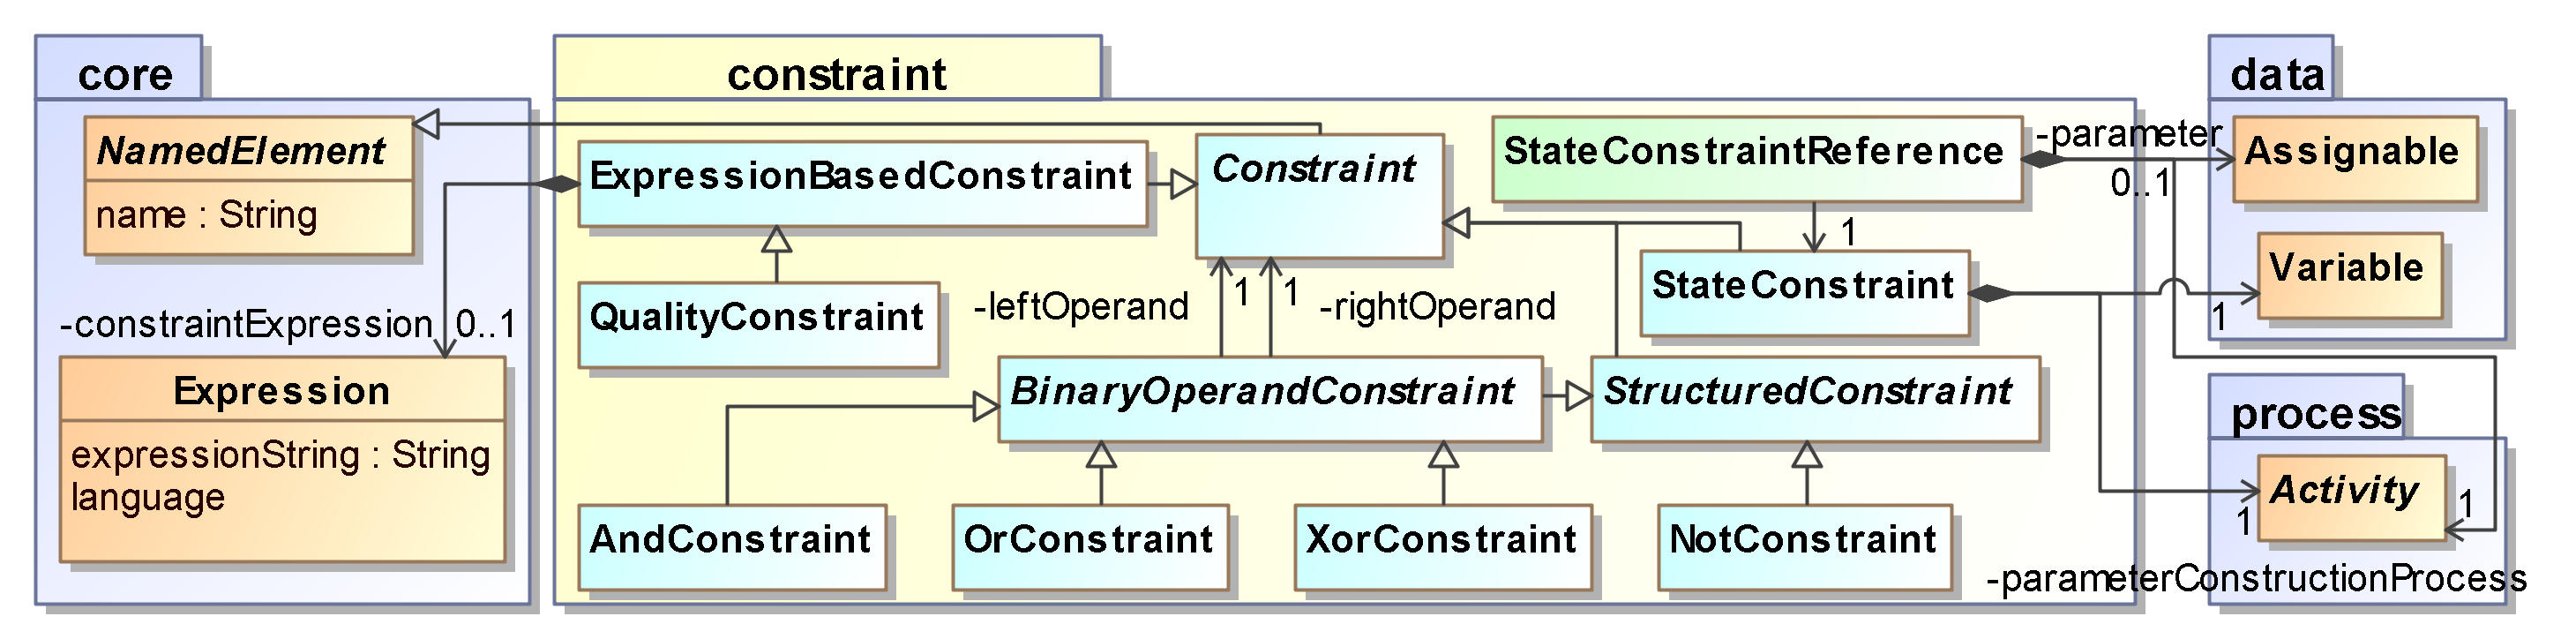
\includegraphics{constraint}
  \caption{The constraint specification elements of URDAD}
  \label{fig:constraintModule}
\end{figure}

The \emph{contract module} of the URDAD metamodel has the modeling constructs used to specify services contracts. The specification of a services contract within the URDAD DSL text grammar is illustrated with the following listing.
\lstset{language=urdad,caption=Specifying a service contract in the textual URDAD DSL syntax.,label=contractTextSyntax}
\begin{lstlisting}[numbers=left,escapechar=|]
ServiceContract enrollForPresentation
{
   FunctionalRequirements receiving Variable enrollForPresentationRequest ofType EnrollForPresentationRequest
   {
      PreCondition enrollmentPrerequisitesMet requiredBy (TrainingRegulator Student) raises EnrollmentPrerequisitesNotSatisfiedException checks constraint enrollmentPrerequisitesForPresentationMet with ValueOf enrollForPresentationRequest
      PostCondition enrollmentProcessPerformed requiredBy (Student Client TrainingRegulator) ensures constraint studentEnrolledForPresentation          with ValueOf studentEnrolledRequest constructedUsing doSequential
         {
            create Variable studentEnrolledRequest ofType StudentEnrolledRequest
            set Query OCL:"studentEnrolledRequest.personIdentifier" equalTo Query OCL:"enrollForPresentationRequest.personIdentifier"                            
            set Query OCL:"studentEnrolledRequest.presentationIdentifier" equalTo Query OCL:"enrollForPresentationRequest.presentationIdentifier"                            
         }  
      PostCondition invoiceIssued ...
    }            
    Request DataStructure EnrollForPresentationRequest 
    {
       has identification presentationIdentifier identifying Presentation
       has identification studentIdentifier identifying Person
       has identification clientIdentifier identifying LegalEntity         
    }
    Result DataStructure EnrollForPresentationResult 
    {
       has component proofOfEnrollment ofType ProofOfEnrollment
       has component invoice ofType Invoice
       has component studyGuide ofType StudyGuide
    }
}
\end{lstlisting}

The contract specification includes pre- and post-conditions, quality requirements and the data structure specifications for the request and result objects of the service. Figure \ref{fig:contractModule} shows the elements of the contract modules of the URDAD metamodel.

\begin{figure}[Htbp]
  \centering
  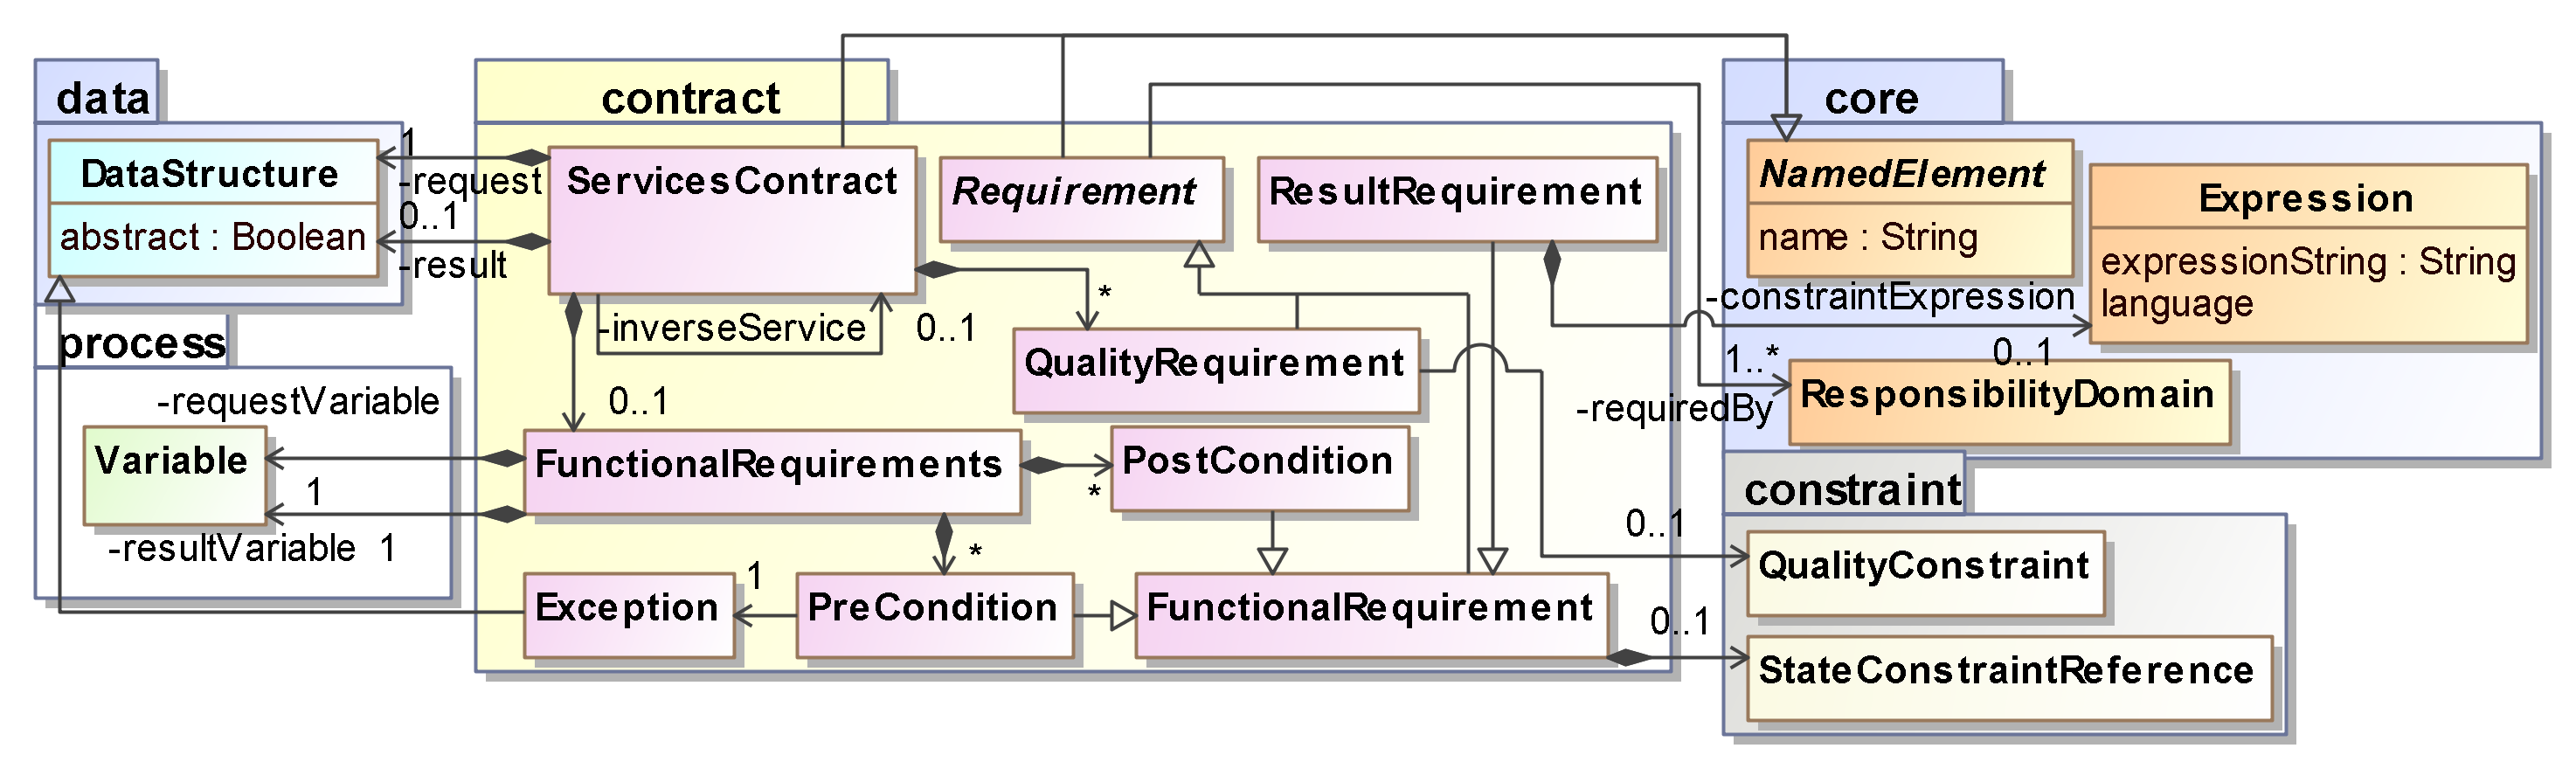
\includegraphics{contract}
  \caption{The contract specification elements of URDAD}
  \label{fig:contractModule}
\end{figure}

The \emph{process module} depicted \ref{fig:processModule} in figure contains the modeling constructs used to specify the process for a service realizing a services contractModule.
 
 This is done via \verb+usedToAddress+ links representing satsifaction links as in  \cite{ramesh_toward_2001}). 

The second aspect of a service is the specification of a process which is assembled from service requests associated with the lower level services contracts used to address the functional requirements of the service. Note that decoupling of levels of granularity via services contracts is enforced. The URDAD metamodel assumes that the selection of concrete service providers for the lower level services is either done by the deployment environment through mechanisms like \emph{dependency injection} or specified during the implementation mapping phase.

The URDAD metamodel also contains explicit modelling constructs for creating and manipulating local process variables,  for handling an exception raised by a lower level service, for raising an exception associated with a pre-condition of the service, and for the return of a computational result. 


\begin{figure}[Htbp]
  \centering
  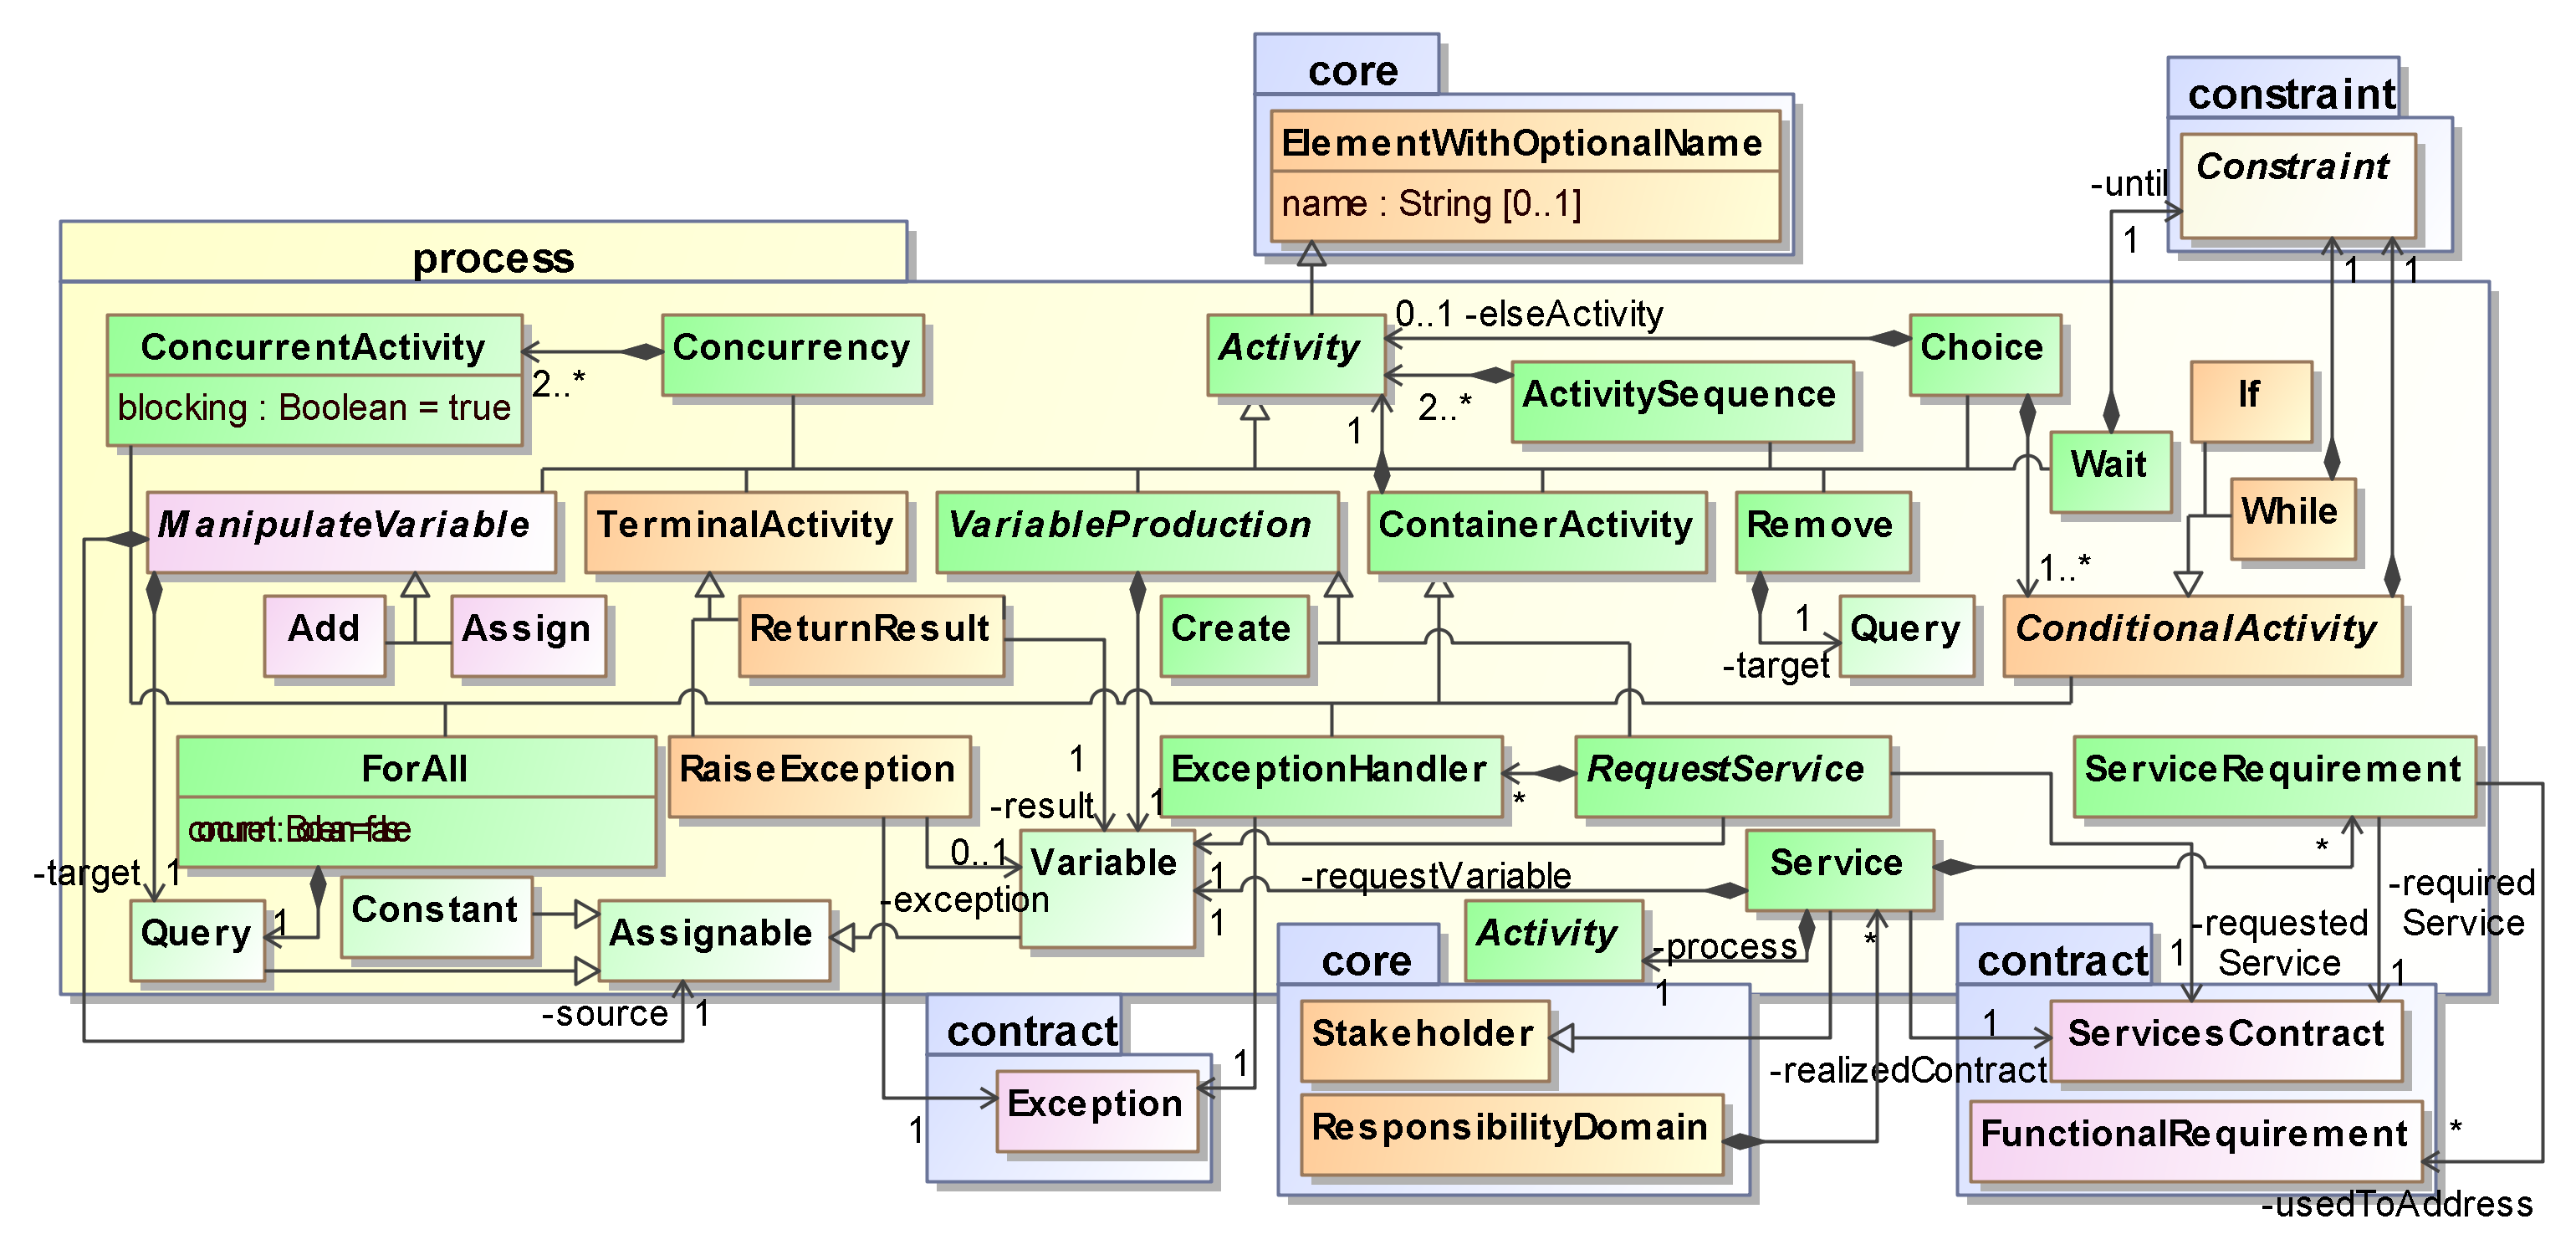
\includegraphics{process}
  \caption{The process definition elements of URDAD}
  \label{fig:processModule}
\end{figure}

The following listing illustrates how a service contract is denoted in the grammar of our URDAD DSL.
\lstset{language=urdad,caption=Specifying a service in the textual URDAD DSL syntax.,label=serviceTextSyntax}
\begin{lstlisting}[numbers=left,escapechar=|]
Service enrollForPresentationImpl realizes enrollForPresentation receiving Variable enrollForPresentationRequest ofType EnrollForPresentationRequest
{
  use checkStudentSatisfiesEnrollmentPrerequisites toAddress (enrollmentPrerequisitesMet)
  use issueInvoice toAddress (financialPrerequisitesSatisfied invoiceIssued) 
  use performEnrollment toAddress (invoiceIssued)
   
  Process doSequential
  {
    create Variable checkStudentSatisfiesEnrollmentPrerequisitesRequest ofType CheckStudentSatisfiesEnrollmentPrerequisitesRequest               
    set Query OCL:"enrollForPresentationRequest.studentIdentifier" equalTo Query OCL:"checkEnrollmentPrerequisitesRequest.studentIdentifier"
    set Query OCL:"enrollForPresentationRequest.presentationIdentifier" equalTo Query OCL:"checkEnrollmentPrerequisitesRequest.presentationIdentifier"
                     
    requestService checkStudentSatisfiesEnrollmentPrerequisites with checkStudentSatisfiesEnrollmentPrerequisitesRequest yielding Variable checkStudentSatisfiesEnrollmentPrerequisitesResult ofType CheckStudentSatisfiesEnrollmentPrerequisitesResult
    choice
    {
      if Constraint enrollmentMeetsPrerequisitesMet OCL:"checkStudentSatisfiesEnrollmentPrerequisitesResult.enrollmentPrerequisitesMet = true"
        doSequential
        {
          ...
          requestService issueInvoice with issueInvoiceRequest yielding Variable issueInvoiceResult ofType IssueInvoiceResult
          {
            on FinancialPrerequisitesNotSatisfiedException raiseException FinancialPrerequisitesNotSatisfiedException
          }
	      ...
          requestService performEnrollment with enrollRequest yielding Variable performEnrollmentResult ofType PerformEnrollmentResult
          
          create Variable enrollForPresentationResult ofType EnrollForPresentationResult
          set Query OCL:"issueInvoiceResult.invoice" equalTo Query OCL:"enrollForPresentationResult.invoice"
          ...                       
          returnResult  enrollForPresentationResult
        }
      else raiseException EnrollmentPrerequisitesNotSatisfiedException
    }
  }
}                 
\end{lstlisting}




%---------------------------------------------------------------

\subsection{URDAD views}
\label{sec:urdadViews}

supplied via text encoding and later via graphical syntax.

%---------------------------------------------------------------

\subsection{Example: Designing URDAD with URDAD}
\label{sec:urdadExample}
by using it to design a service oriented analysis and design methodology. If the process is internally consistent it needs to generate itself. 


%---------------------------------------------------------------

\todo{Fritz: mention adapters to existing legacy}

\todo{Fritz: Add that one of the core challanges is to have requirements specialists make the paradigm shift to specify requirements in terms of services contracts for reusable services\cite{haines_impact_2007}. In practice we have found that URDAD assists significantly on that front.}


\section{Model quality}

\todo[color=red!40]{Fritz: Remove the requirements aspects after ensuring everything is in the requirements section}

In order to identify the stake holders who have an interest in the model and who may have functional and quality requirements for the model
Stakeholders and what they use the model for
\begin{itemize}
  \item Developers to perform implementation mapping
  \item Architectects to 
\end{itemize}


\cite{lange_managing_2005,lange_improving_2006}.


Emphasize that model a functional model, bot addressing non-functional (quality requirements) of system

\begin{itemize}
  \item \emph{testability} measured as fraction of non-testable requirements.
  \item \emph{traceability} measured as fraction of requirements which are not related to the stake holder who requires them, fraction of activities which are not traceable to the functional requirement they aim to address, 
  \item \emph{complexity} based on number and complexity of services with complexity of service necessarily related to Mcabe (cyclomatic) complexity - not sure that URDAD addresses this.
  \item \emph{cohesion} - will be interesting to try and find a measure for cohesion in the service oriented world.
  \item \emph{reuse} - number of
  \item \emph{coupling} - URDAD enforces decoupling across levels of granularity in both, the process and the metamodel.
  \item \emph{completeness}
  \item \emph{non-ambiguous}
\end{itemize}


MDA requires model to be technology neutral.

completeness can be checked relative to a responsibility domain, i.e. the processes for all services within my responsibility domain specified as assembled from either specified services from my responsibility domain or as services sourced from another responsibility domain.

methodology churns out intermediate levels of granularity assisting to constrain model complexity by 


model quality supported through validation against metamodel constraints

How much of the model quality measurement can be automated?

Because model in problem domain, domain experts can validate, improving model quality

URDAD trades off pure requirements against manageable requirements

\cite{graham_requirements_2008} do Model validation by requiring that every goal (pe/post-condition) addressed by a message exchange (service request) and that all messages are associated with achiving a goal.

A direct implementation mapping will transfer many of the design qualities onto the code (modifiability, pluggability, reuse, ...)

because requirements and design are arch and techn neutral, stakeholders (business) can understand them and validate them, improving quality


Sifiso:
To an extent quality can be seen as mesure of value that can be extracted from the model, these can be mesured by:-

(1) The level of abstraction it provides
(2) Understandibilty 
(3) Accuracy 
(4) Predictiveness
(5) Cost -Inexpesiveness 
\cite{selic_pragmatic_mdd_20003}



\subsection{Process stakeholders and their quality requirements}

According to both Crosby and Demig quality is defined in terms of custumer satisfaction. Looking at the URDAD process and trying to answer the 
question: To what extend does the URDAD process fullfil the requirements of the stake holders that have an interest in it. 

\begin {itemize}
 \item Give a scenairo where URDAD is bieng applied
 \item Look at the stake holders who have interest in the URDAD process 
 \item Identify their requirements requirements
 \item See and disscuss how those requirements are best address by the process
\end {itemize}

\begin {itemize}
 \item Discuss the URDAD process incoparated in to a Software Development Methodology
 \item How URDAD can be used with other to solve specific problem(Service Oriented),
  while a different methodology is bieng used fro the rest of the project. How can this contribute to quality ?
  Compare URDAD to other methodologies, from a quality point of view.
\end {itemize}


\cite{berard_what_1995}

Stake holders:
\begin{itemize}
  \item Project management (measurability, repeatability, estimatability)
  \item Requirements specialists (ease of use, simple process, defined process activities, defined inputs and outputs, tool support)
  \item Business (low cost, trainable, grow in islands)
\end{itemize}


\begin{itemize}
  \item Process measurability
  \item Repeatability
  \item Defined inputs and outputs
  \item Clearly specified tasks with defined activities
  \item Process consistency (URDAD generates itself)
\end{itemize}

Can apply process to a sub-world, decouples from higher and lower level granularities via contracts

Could introduce more abstract qualities and things the process must have to realize these, e.g. \emph{usability} affected by many of these

CMM requires process definition


\subsection{Internal process consistency}

\todo[inline,color=blue!40]{Fritz: Reuse sounds to me like both, a process and a model quality}

Here show that if you use URDAD to design an analysis and design methodlogy, you will get URDAD. Feed additional concepts into URDAD.

Here identify the stakeholders in both, the process and the outputs of the process and their quality requirements.


\subsection{Internal process consistency}

Here show that if you use URDAD to design an analysis and design methodlogy, you will get URDAD. Feed additional concepts into URDAD.

process assists in improving quality of requirements by forcing certain questions


\section{Related work \label{sec:relatedWork}}

The URDAD methodology provides a services-oriented methodology for generating a semi-formal analysis and design model representing MDA's PIM and supporting test and implementation generation. \cite{iacob_model-driven_2008} discuss an alternative approach. Business Rules are specified using OMG's {\em Semantics for Business Vocabulary and Rules} (SBVR) to service specification and orchestration and BPEL process specifications are generated using MDA tools. Processes are assembled from services which are related to business rules. This is similar to our satisfiability links specifying the services used to realize the different functional requirements.

The URDAD DSL allows for the specification of textual and graphical grammars through which the URDAD model is populated. An alternative approach is to define a separate metamodel for the use case narrative and to transform the narrative model requirements model \cite{hoffmann_towards_2009,osis_transforming_2010}. This approach introduces the complexities of having to transform from the narrative to the UML model and requires extensive consistency checks between the narrative and the UML models.

\cite{asnina_computation_2010} stress the need of modelling in the problem domain as well the benefits of accumulating requirements within a single model. Services are grouped into feature sets which are related to responsibility domains. Functional requirements are decomposed across levels of granularity and higher level processes are orchestrated across lower level services. They define the notion of functionals with cause and effect which can be related to the concept of a services contract. In addition they provide a {\em topological functional model} (TFM) for mapping technology neutral service requirements onto available concrete services pool. The TFM is independent of the modelling technique and can be applied to an URDAD model. 

In the {\em Requirements Driven Design Automation} methodology (RDDA) \cite{cardei_model_2008} one encodes requirements specifications in SYSML diagrams. The SYSML model is enriched with semantic descriptions after which the model is transformed to the {\em One Pass to Production} (OPP) design language, the ODL. ODL is an OWL based ontology from which the requirements are validated for consistency and completeness. The approach is, however, structure focused with little emphasis on services contracts and recursive orchestration of higher level services from lower level services.


\section{Conclusions and outlook}

In this paper we identified the stakeholders in the analysis and design methodology and the resultant requirements and technology neutral process design model and their quality requirements. We related these quality requirements to quality drivers and measures which can be applied within a services-oriented approach. We then identified that subset of quality drivers which has been embedded within the URDAD process and pointed out how some of these are enforced by the URDAD metamodel.

One of the practical benefits of the URDAD methodology is that it assists requirements engineers to make the paradigm shift\cite{haines_impact_2007} to defining stand-alone services contracts and to assemble processess from abstract, reusable, stateless services with the concrete service providers either selected during the implementation mapping phase or alternatively provided by the execution environment through mechanisms like real-time service provider selection and dependency injection.

Future work includes the specification of a graphical grammar making the domain specific language for URDAD accessible to requirements engineers like business analysts and the specification and development of quality assessment tools which can be used to either report quality measures or provide real time quality guidelines to modelers.

\bibliographystyle{plain}  %%abbrv
\bibliography{../../bibliography}

\end{document}
